\chapter{Allgemein Bluetooth}
\label{ch:general}

\section{Geschichte}

\begin{wrapfigure}{r}{0.4\textwidth}
	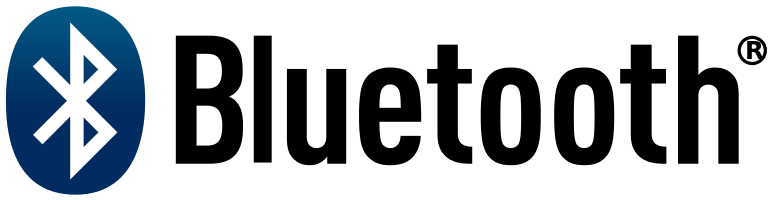
\includegraphics[width=1.0\linewidth]{images/bluetooth_logo.png}
	\caption[Bluetooth Logo]{Bluetooth Logo (Quelle: \fullcite{Bluetooth_Wikipedia_2015-04-17})}
\end{wrapfigure}
Die Voraussetzung für das heutige weit verbreitete Bluetooth, schuf der Physiker Dr. Johan Ullman.
Bereits 1989 präsentierte er seine erste Erfindung für ein kabelloses Headset.\footcite{Bluetooth_Wikipedia_2015-04-17}

1994 wurden die Erfindungen von der Firma \textit{Ericsson Mobile}\footcite{Ericsson_2015-04-17} aufgenommen.
Mit Hilfe von Intel, Nokia, IBM und Toshiba wurde im Jahr 1998 die neue Technologie von der \gls{sigLabel} veröffentlicht.
\footcite{Bluetooth_Special_Interest_Group_Wikipedia_2015-04-17}\footcite{The_history_of_Bluetooth_Ericsson_History_2015-04-17}

Die Bezeichnung der Technologie lautete während der Entwicklung \gls{mclLabel}.
Ein Mitentwickler war jedoch von \textit{Harald Bl{\aa}tand}, einem ehemaligen König von Dänemark des 10. Jahrhunderts, so begeistert, dass die Bezeichnung der Technologie nach des Königs Namen geändert wurde: Blauzahn bzw. Bluetooth.
Bl{\aa}tand war bekannt für die Vereinigung von Skandinavien, genau so wie Bluetooth für eine einheitlich drahtlose Verbindung bekannt werden soll.
Das Logo von Bluetooth zeigt die Initialien von Harald Bl{\aa}tand (HB) in einer alten Schrift (in der Runenform).

Im Jahr 2000 wurde das erste Headset mit Bluetooth verkauft.

\section{Technische Spezifikationen}
\label{sec:general_specs}
% Im folgenden \secref{sec:general_specs} stammen mehrere Informationen aus Wikipedia.\footcite{Bluetooth_Wikipedia_2015-04-17}
% Im diesem \secref{sec:general_specs} folgen Informationen zu Versionen und Geschwindigkeiten (\subsecref{subsec:versions_speed}), Physikalische

\subsection{Versionen und Geschwindigkeiten}
\label{subsec:versions_speed}
Die Bluetooth-Version 1.0 wurde 1999 veröffentlicht, doch sie beinhaltete noch viele Fehler.

Über die Jahren haben sich vier Hauptversionen durchgesetzt:\footcite{Bluetooth_low_energy_Wikipedia_2015-04-17}\footcite{Our_History_Bluetooth_Technology_Website_2015-04-17}
\begin{table}[H]
% style
\small\sffamily\renewcommand{\arraystretch}{1.4}
% caption
\captionabove{Bluetooth Geschwindigkeiten mit Versionen}
\begin{tabular}{llrrl}
\toprule
	Version & Bezeichnung & Geschw. & effektive Geschw.  & Jahr\\
\midrule
	1.2 & \gls{brLabel} & 1\,Mbit/s & 0.7\,Mbit/s & 2003 \\
	2.0 & \gls{edrLabel} & 3\,Mbit/s & 2.1\,Mbit/s & 2004 \\
	3.0 & \gls{hsLabel} & 24\,Mbit/s & 2.1\,Mbit/s & 2009\\
%	4.0 & \gls{hsLabel} & 24\,Mbit/s & -  & 2010 \\
	4.0 & \gls{leLabel} Erweiterung & 1\,Mbit/s &  0.27\,Mbit/s & 2010 \\
\bottomrule
\end{tabular}
\end{table}
% \footcite{How_Bluetooth_Creates_a_Connection_HowStuffWorks_2015-04-17}



\subsection{Physikalische Übertragung}
Die Übertragung des klassischen Bluetooth erfolgt auf den Frequenzen 2.4 bis 2.480\,GHz, welche in 79 Kanäle à 1\, MHz unterteilt werden.
Bei \gls{bleLabel} stehen pro Kanal 2\, MHz zur Verfügung, was die Anzahl Kanäle auf 37 reduziert.

Es wird die Funktechnologie des \textit{frequency-hopping spread spectrum} verwendet.
Dabei wird jedes Paket auf einem anderen Kanal versendet.
Der Kanal wird 1\'600 mal pro Sekunde gewechselt.\footcite{Bluetooth_Wikipedia_2015-04-17}

Durch das \textit{frequency-hopping} ergeben sich drei wesentliche Vorteile:\footcite{Frequency-hopping_spread_spectrum_-_Wikipedia_2015-04-17}
\begin{itemize}
	\item \textbf{Anzahl der Verbindungen:} Die Übermittlung eines Pakets blockiert einen Kanal nur für kurze Zeit.
		Anschliessend kann der Kanal bereits wieder für die nächste Übertragung verwendet werden.
		So steigt die Effizienz über die ganze Bandbreite.
	\item \textbf{Abhörsicherheit:} Durch das Wechseln der Kanäle, wird das Abhören der Verbindung massiv erschwert, da dem Angreifer die Reihenfolge der verwendeten Kanäle nicht bekannt ist.
	\item \textbf{Rauschen:} Durch die Wechsel wird das Rauschen unterdrückt.
\end{itemize}

\begin{framed}
	\textbf{Information:} Das \textit{frequency-hopping spread spectrum} wurde von Hedy Lamarr, einer österreich-amerikanischen Frau, während des zweiten Weltkrieges erfunden. Sie war zudem eine erfolgreiche Schauspielerin.\footcite{Hedy_Lamarr_Wikipedia_2015-04-27}
\end{framed}


\subsection{Klassen (Reichweite)}
Bluetooth-fähige Geräte können abhängig ihrer Reichweite in folgende drei Klassen eingeteilt werden:
\begin{itemize}
	\item \textbf{Klasse 1:} Distanz bis zu 100\,m
	\item \textbf{Klasse 2:} Distanz bis zu 10\,m
	\item \textbf{Klasse 3:} Distanz bis zu 1\,m
\end{itemize}
Die meisten Geräte (wie Mobiltelefone, Computers, Headsets, etc.) entsprechen der \textit{Klasse 2}.



\section{Kommunikation}
Bluetooth ist ein paketbasiertes Protokoll mit einem \textit{Master-Slave} Prinzip. Dieses Prinzip wird nun kurz erläutert.

Pro Netzwerk (\textit{Piconet}) kann ein Master mit bis zu sieben aktiven Slaves kommunizieren.
Der Master definiert welcher Slave wann antworten darf (meist via \gls{glos:roundRobinLabel}).
Folglich muss ein Slave immer aktiv zuhören, um seinen zugeteilten Sende-Slot nutzen zu können. Die Funktion des Masters ist weniger aufwändig als die eines Slaves.
Nebst den aktiven Slaves, können bis zu 255 Slaves in den \textit{PARK}-Modus (siehe \cref{subsec:energymode}) gesetzt werden, aus dem sie jederzeit reaktiviert werden können.
\footcite{Piconet_-_Wikipedia_2015-04-18}


Die Rollen (Master und Slave) können auch getauscht werden.
Dies geschieht zum Beispiel, wenn via Headset eine Verbindung zu einem Mobiltelefon aufgebaut wird:
Zuerst übernimmt das Headset die Rolle des Masters, übergibt die aber sobald wie möglich dem Telefon.

Der \textit{Master} definiert für alle seine Slaves den \gls{glos:clockLabel} ($312.5\,\mu s$).
Jeweils zwei Clocks ergeben einen \textit{Slot}.
Der Master beginnt eine Sendung immer auf einen geraden Slot.
Für die Slaves stehen die ungeraden Slots als Start einer Sendung zur Verfügung.

Ein Paket kann ein, drei oder fünf Slots lang sein.

Bluetooth definiert mehrere Piconets zu einem \textit{Scatternet}.
Dabei kann ein Gerät, nebst maximal einer Master-Rolle, mehrere Slaves-Rollen in verschiedenen Piconets belegen.

\subsection{Asynchron und synchrone Kommunikation}
Die Kommunikation kann entweder \gls{scoLabel} oder \gls{aclLabel} erfolgen.
\gls{scoLabel} wird für den Austausch von Sprachdateien (64\,kbit/s) verwendet, wobei bis zu drei duplex Verbindungen zur gleichen Zeit aktiv sein können.
\gls{aclLabel} setzt ein speicherndes Verhalten der Endgeräte voraus (analog zum Internet). Die asynchrone Verbindung erlaubt eine \textit{symmetrisch} (mit 2 x 433,9\,kbit/s) und eine \textit{asymmetrisch} (mit 706,25 und 57,6\,kbit/s) verteilte Übertragungsgeschwindigkeit.
\footcite{Nahfunktechnik_in_Smartphones_FAQ_cio.de_2015-04-24}


\subsection{Energiesparmodi}
\label{subsec:energymode}
Da klassisches Bluetooth bereits seit Beginn eine stromsparende Nutzung anvisiert, gibt es folgende drei Energiesparmodi:
\begin{itemize}
	\item \textbf{HOLD-Modus:} Hier kann vorläufig eine Abwesenheit mitgeteilt werden, während der keine Daten empfangen werden können. So können während dieser Zeit bewusst andere Aufgaben erledigt werden.
	\item \textbf{SNIFF-Modus:} Im SNIFF-Modus werden periodische Aktivitäten reduziert, z.B. kann der Kanal nur noch alle 500\,ms abgehört werden.
	Dieser Modus wird sehr oft eingesetzt, um den Energieverbrauch zu senken.
	\item \textbf{PARK-Modus:} Das Gerät bleibt zwar synchronisiert, kann jedoch während diesem Modus nicht am Datenverkehr teilnehmen. Dieser Modus wird in der Praxis kaum verwendet.
\end{itemize}


\subsection{Verbindungsaufbau}
\label{sec:connectionSetup}
Sobald sich ein Gerät im \textit{Discoverable Mode} befindet, sendet es auf Anfrage folgende Daten: \textit{Name des Gerätes}, \textit{Klasse des Gerätes}, \textit{Liste der unterstützten Services} und \textit{weitere technische Informationen}.

Jedes Bluetooth-fähige Gerät kann die Informationen eines anderen Gerätes im \textit{Discoverable Mode} verlangen und direkt eine Verbindung zu diesem aufbauen.

Konkret wird jedes Gerät mit einer 48-Bit Adresse identifiziert. Der Benutzer sieht jedoch lediglich die nicht eindeutigen und selbst definierbare Bezeichnung. Viele Hersteller setzen diese Bezeichnung standardmässig auf die Modellbezeichnung, was dazu führt, dass oft mehrmals gleiche Bezeichnungen angezeigt werden.

Um nun eine Verbindung herzustellen, wird das gewünschte Gerät in den \textit{Scan-Modus} gesetzt.
Dabei wird auf 32 Hop-Frequenzen, während 2.56\,s nach möglichen Slaves gesucht. Dazu werden sogenannte Inquiry-Messages (Erkundigungsnachrichten) verschickt.
Wenn Slaves gefunden werden, wird ihnen per Page-Messages auf 16 Kanälen eine Verbindung angeboten.

Falls keine Verbindung zustande kommt, wird der Suchprozess auf weiteren 16 Hop-Frequenzen fortgefahren.

Der durchschnittliche Verbindungsaufbau dauert 1.28\,s.\footcite{Bluetooth_de_Wikipedia_2015-04-18}

Ab Bluetooth 3.0 ist zusätzlich ein \gls{glos:connectionlessCommunicationLabel} möglich.

Der Verbindungsaufbau für \gls{bleLabel} wird in \cref{subsec:bleConnectionSetup} erläutert.

\section{Profile}
Bluetooth definiert verschiedene \textit{Bluetooth Profile} um Daten zu übertragen.
Für einen erfolgreichen Datenaustausch müssen jeweils alle Geräte das zu verwendende Profil unterstützen.

Selbstsprechende Beispiele für häufig verwendete Profile sind \gls{hspLabel}, \gls{gavdpLabel} oder  \gls{hdpLabel}.\footcite{List_of_Bluetooth_profiles_Wikipedia_2015-04-27}

Eine vollständige Sammlung der standardisierten Profilen ist auf der Website von Bluetooth vorhanden.\footcite{Profiles_Overview_Bluetooth_Development_Portal_2015-04-27}


\section{Sicherheit}
In diesem Abschnitt wird auf verschiedene Sicherheitsmerkmale eingegangen.

\subsection{Pairing, Bonding}
Viele Service benötigen, nebst einem Verbindungsaufbau, ein erfolgreiches \textit{Bonding}, das durch ein \textit{Pairing} (Koppelung) zustande kommt.
Dabei wird initial die Identität der beiden Geräte verifiziert, sodass künftig Service genutzt werden können, ohne dass eine Benutzerinteraktion erforderlich ist.

Seit der Bluetooth Version 2.1 wird das \gls{sspLabel} standardmässig verwendet. Es unterstützt folgende vier Modi:\footcite{Bluetooth_Wikipedia_2015-04-17}
\begin{itemize}
	\item \textbf{Just works:} Es wird keine Interaktion des Benutzers benötigt. Dies wird oft für Geräte ohne \gls{glos:ioLabel} Möglichkeiten eingesetzt, und bietet keinen Schutz gegen \gls{mitmLabel}-Angriffe.
	\item \textbf{Numeric Comparison:} Auf den Displays beider Geräte wird eine Zahl angezeigt, die übereinstimmen muss. So wird sichergestellt, dass kein \gls{mitmLabel}-Angriff vorliegt.
	\item \textbf{Passkey Entry:} Hier muss mindestens eine \gls{pinLabel} des einen Gerätes auf dem anderen eingegeben werden. Somit wird \gls{mitmLabel}-Angriff verunmöglicht.
	\item \textbf{\gls{oobLabel}:} Diese Methode wird meistens über \gls{nfcLabel} realisiert.
		\gls{oobLabel} schützt nicht per Definition vor \gls{mitmLabel}-Angriffen, aber erschwert diese erheblich. Der Angreifer muss ein weiteres Medium abhören können, was z.B. bei \gls{nfcLabel} nur in extrem kleinem Radius möglich ist.
\end{itemize}


\subsection{Sicherheitsmodi}
Im Bluetooth-Standard werden vier Sicherheitsmodi definiert:\footcite{Security_Bluetooth_Development_Portal_2015-04-24}
\begin{itemize}
	\item \textbf{Mode 1 - Non-Secure:} In diesem Modus werden keine Sicherheitsvorsichtsmassnahmen unterstützt.
	\item \textbf{Mode 2 - Service-Secure:} In diesem Modus erfolgt die Sicherheit auf dem \textit{Application Layer} des Services.
	\item \textbf{Mode 3 - Link-Secure:} Dieser Modus unterstützt eine Authentifizierung auf dem \textit{Link Layer}.
	\item \textbf{Mode 4 - Link-Secure encrypted:} Dieser Modus unterstützt ebenfalls die Authentifizierung auf dem \textit{Link Layer}, wobei hier der Schlüssel-Austausch explizit verschlüsselt erfolgen muss.
\end{itemize}

\newpage
\subsection{Verschlüsselung}
Beim klassischen Bluetooth wird die Stromchiffre \textit{E0} (128-Bit) verwendet.\footcite{E0_cipher_Wikipedia_2015-04-27}
Dazu werden folgende fünf Werte benötigt:
\footcite{LE_Security_Bluetooth_Development_Portal_2015-04-25}
\footcite{Bluetooth_Communication_Hybrid_Encryption_2015-04-25}
\footcite{BluetoothSecurity_Washington_2015-04-25}

\begin{table}[H]
	% style
	\small\sffamily\renewcommand{\arraystretch}{1.4}
	% caption
	\captionabove{Verschlüsselungswerte}
	\begin{tabular}{p{0.25\linewidth}lp{0.5\linewidth}}
		\toprule
		Parameter & Länge & Beschreibung \\
		\midrule
		BD\_ADDR & 48 Bit & Entspricht einer eindeutigen Geräte-Adresse, die durch das \gls{ieeeLabel} definiert wird.\\
		\gls{pinLabel} & bis zu 128 Bit & \gls{pinLabel} der auf beiden Geräten übereinstimmen muss. Entweder hat eines der Geräte einen fix hinterlegten \gls{pinLabel} oder er kann selbst definiert werden.\\
		Link Key & 128 Bit  & Wird jeweils von zwei paired Geräten und für die Authentifikation verwendet. Wird auch \textit{Private Authentication Key} genannt.\\
		Private Encryption Key & 8 -- 128 Bit & Pro Übertragung (Session) wird ein Encryption Key aus dem Link Key abgeleitet. Die Länge wird durch die zwei Geräte festgelegt, wobei beide ein Minimum sowie ein Maximum definieren. Falls sich keine Übereinstimmung ergibt, muss abhängig des Services entschieden werden, ob trotzdem eine Verbindung zustande kommen darf. \\
		RAND & 128 Bit & Der RAND-Wert wechselt häufig und wird für Key Generierungen verwendet.\\
		\bottomrule
	\end{tabular}
\end{table}

Mit Hilfe des \gls{pinLabel}'s, des RAND's und der BD\_ADDR wird ein \textit{Initialization Key} berechnet.
Für die Authentifizierung müssen beide Geräte eine zufällige Zahl des anderen korrekt berechnen können.
Bei Erfolg wird die BD\_ADDR vom \textit{Service Manager} des Gerätes als authentifiziert abgelegt.
Bei Misserfolg erfolgt eine neuer Versuch, nachdem eine exponentielle steigende Wartezeiten abgelaufen ist.

Bei einer bevorstehenden Datenübermittlung, wird geprüft ob der Kommunikationspartner bereits einmal authentifiziert wurde. Wenn nicht, wird die Authentifizierung durchgeführt.
Falls bereits früher eine Authentifizierung stattgefunden hat, wird ein gültiger Link Key für die effektive Verschlüsselung der Daten ausgemacht.

Bei \gls{bleLabel} erfolgt die Verschlüsselung via \gls{aesccmLabel}, ebenfalls mit 128 Bit.

\subsection{Error Correction}
Die Daten werden entweder beim klassischen Bluetooth mit \gls{fecLabel}\footcite{Forward_error_correction_Wikipedia_2015-04-27} oder bei bei \gls{bleLabel} mit \gls{crcLabel}\footcite{Cyclic_redundancy_check_Wikipedia_2015-04-27} auf Übermittlungsfehler überprüft.
